\documentclass{article}
\usepackage[utf8]{inputenc}

\title{GU-Makro-Formler}
\author{orts }
\date{April 2016}

\usepackage{natbib}
\usepackage{graphicx}

\begin{document}

\maketitle

\section{Introduction}
Formler för makroteori. Går igenom och förklarar alla relevanta formler. 



\section{Conclusion}
``I always thought something was fundamentally wrong with the universe'' \citep{adams1995hitchhiker}

\section{Långa sikten F2-F11}
\title{Föreläsning 1}

Under krisen 2008 så sjönk BNP per capita kraftigt. Idag har den återhämtat sig så att den är på samma nivå som 2007. 

$$
    \Delta \ ln \ Z = \Delta \ln  X + \Delta \ ln Y - \Delta \ ln Q
$$
Förenkling vid förändring. Gäller vid följande. 
$$
Z = \frac{X*Y}{Q}
$$

Idag har Sverige överskott i bytesbalansen. 

Det existerar tre sätt att bestäma värdet som produceras inom ett lands gränser. 

\begin{enumerate}
    \item Användning. Summa utgifter för nya varor/tjänster för slutgiltig användnign minus import. 
    \item Produktion: summa förädlingsvärde.
    \item Inkomst: summa kaptial- och arbetsinkomster. 
\end{enumerate}

\begin{equation}
    BNP = \ Y\ = \ C + I + C^G + I^G + X - IM 
\end{equation}

Bruttonationalinkomsten, BNI: 

$$
BNI = Y + Y^F \ (Y^F: landets \ faktorinkomster.) 
$$
Faktorinkomster: ersättning till arbete och kapitel som "ägs" av landets medborgare. Det vill säga avkastning från utlandet. 

Dissponibel buruttonationalinkomst, DBNI: 

$$
DBNI = Y + Y^F + Tr^F 
$$


\textbf{Bytesbalansen}: Denna summerar flödet mellan oss och omvärlen. 

$$
Bytesbalansen = NX + Y^F + Tr^F
$$
Har vi överskott i vår bytesbalans så kan detta investeras, dvs lånas ut till andra länder. Om detta är negativt så måste vi låna från de länder som har överskott. 


Nominell BNP = löpande priser.
Real BNP = satt mot ett basår. 
\par \noindent
Tillväxttakt är $g_{t+1}$

\vspace{5mm}


\title{Föreläsning 2}
\vspace{5mm}\par

Sveriges tillväxt startade i mitten på 1800-talet. 

\textbf{Kort sikt < 2år}: Löner och priser är fasta. 

\textbf{Lång sikt 4-5år}: Löner och priser anpassar sig till jämviktsvärden. 

På kort sikt så är konjukturläget det intressanta: inflation, ränta, arbetslöshet, stabeliseringspolitik och budgettunderskott. 

\begin{enumerate}
 \item MPK = kaptialets marginalprodukt. 
 \item MPL = arbetets marginalprodukt. 
\end{enumerate}

\textbf{Prdoutktionsfunktionens egenskaper:}
\begin{enumerate}
 \item Marginalprodukterna är positiva
 \item Marginalprodukterna är avtagande
 \item Konstant skalavkastning
\end{enumerate}

Produktionsfunktion: $$ Y = F(K,N) $$
$$ Y = K^{\alpha}N^{1-\alpha}$$

E = teknisk nivå. 

$$ Y = F(K,EN)$$

\textbf{Jämviktssysselsättning (natrulig)}:
$$N^n = (1-u^n)L $$

L = arbetskraft. 

\begin{itemize}
    \item Långsiktig tillväxt är viktigare än konjukturläget för genomsnittlig inkomst.
    \item Produktionsfunktionen visar producerad kvantitet för given teknisk nivå, kaptialstock, och antal arbetare. 
\end{itemize}

\par
 
 \vspace{5mm}
 \title{Föreläsning 3}
 \vspace{5mm}
 
\par \noindent
Köpkraft = $\frac{W}{P}$, nominell lön delat med prisnivån.\par \noindent
Inverterad efterfrågefunktion: $P_i = P(Y_i,P,Y)$ \vspace{5mm} \par \noindent

Priselasticitet: $$\frac{P_i*dY_i}{dP_i*Y_i}$$

Det genomsnittliga priset: 
$$
P = (1-\mu)MC = (1-\mu)\frac{W}{MPL}
$$

\textbf{Sluten ekonomi: Inkomst = produktion}
Det är köpkraften hos befolkningen som är det viktiga. Detta medför följande: 

$$
 \frac{W}{P} = \frac{MPL}{1+\mu}
$$
Om konkurrensen mellan företag ökar så minskar $ \mu$. \par \noindent

\textbf{Löneandel}: Denna är total lönesumma / nominell BNP 

$$
\frac{WN}{PY} = \frac{1-\alpha}{1+\mu}
$$

På lång sikt så når kapital per arbetare $ \frac{K}{EN} = k $ ett stabilt läge, steady state. 

\textbf{Komihåg till tenta att förklara alla modeller och formler!}

Löneandelen har legat relativt konstant under flera decennier. På ca 1/3. 
Lönesprdningen har ökat, detta kan knytas till automatiseringen. 

\vspace{5mm}
\title{Föreläsning 4} \par \noindent
\vspace{5mm}

$i_t$ är den nominella räntan mellan två perioder. Inflation är hur mycket priset förändras. Det vill säga förändringen i pris från en period till en annan. 
\textbf{Inflation: }
$$
\pi_{t+1} = \frac{P_{t+1}-P_t}{P_t}
$$

Relaränta är ungefär: $r_{t+1} \approx i_t - \pi_{t+1}$

Netto investering: 
$$
K_{t+1} - K_t = I_t -\delta K_t 
$$

\textbf{Optimala kaptialstcken: }
$$
\frac{MPK_{t+1}}{1+\mu}-\delta = r_{t+1}
$$
Ovanstående ekvation säger oss att; Det vi tjänar på att utöka kaptialstocken minus förtäringen på kapitalstocken måste vara lika med priset vi förväntas att betala för det. 


\textbf{Investeringsfunktion:} $I = I(Y^e,K,r)$

\vspace{5mm}
\title{Föreläsning 5}
\vspace{5mm}
\par \noindent

\textbf{Konsumption:} Denna bestäms av inkomsten idag, konsumtionen idag och inkomst i nästa period. 

$$
C_2 = Y^l_2 + (1+r)(Y^l_1-C_1)
$$

$$
\frac{U'(C1_)}{U'(C_2)} = \frac{1+r}{1+\rho}
$$
Den subjektiva räntan $ \rho $ bestämmer hur vida personen annser att det är mer värdefullt att spendera pengar i denna perioden jämfört med nästa. 

\textbf{Konsumptionfunktion:} $ C = C(Y,Y^e,r,A)$

Om den reala räntan ökar så vill befolkningen öka sitt sparande också, då du får mer för dina sparade pengar. Med ökad ränta så sjunker konsumtion och investeringar. 

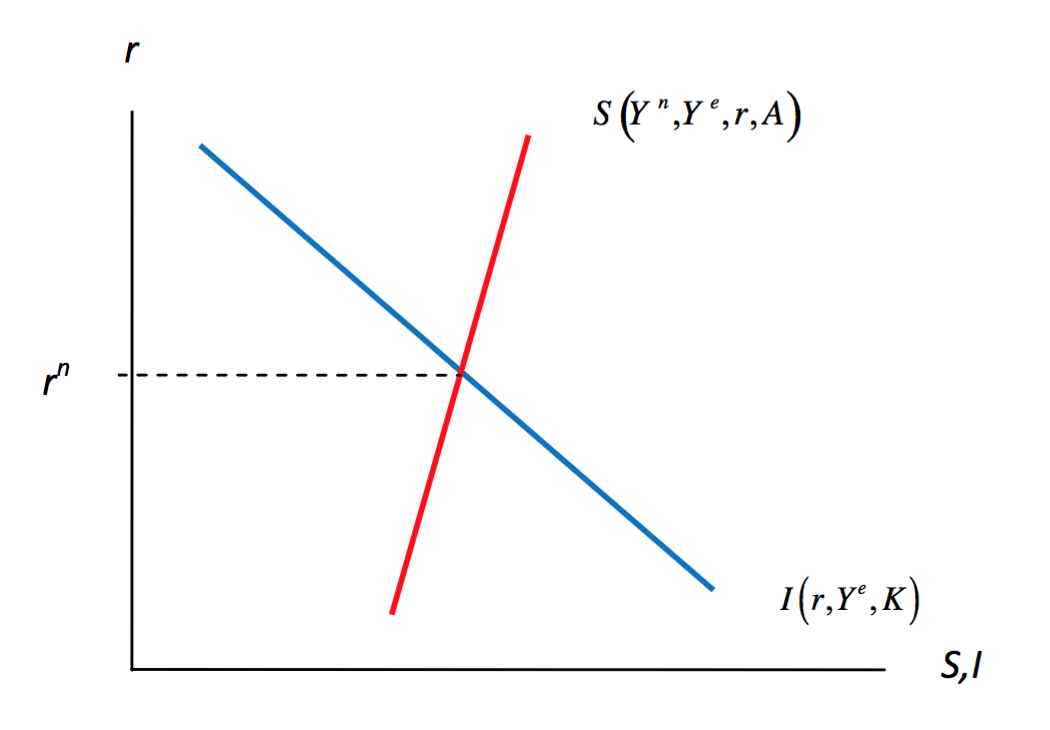
\includegraphics[scale=0.4]{skarm2}

\vspace{5mm}
\title{Föreläsning 7}
\vspace{5mm}
\par \noindent

Den optimala kapitalstocken är också villkor för den långsiktiga jämviktsnivån. 
Genom att ta fram Kaptialets marginalprodukt och sätta in så får vi ut $K^*$.  Detta på lång sikt. På kort sikt kan vi endast kolla på hur det förändrar $MPK \ och \ MPL$. 
Produktionen på lång sikt tar vi fram på liknande vis. Den ges av: 

$$
Y^* = (K^*)^{\alpha}(EN)^{1-\alpha}
$$

Den långsiktiga realräntan = subjektiva diskonteringsräntan.
\par
En sluten ekonomi med konstant befolkning och teknisk nivå. $ \Rightarrow $ varken produktion eller konsumtion kan växa på lång sikt. \par

I en långsiktig jämvikt har vi ingen tillväxt. 

Från ekvationen: 
$$
Y^* = (\frac{\alpha}{(\rho+\delta)(1+\mu)})^{\frac{\alpha}{1-\alpha}}EN
$$

Så här kan det se ut över tid om kaptialstocken eller liknande minskar kraftigt, snabbt: 


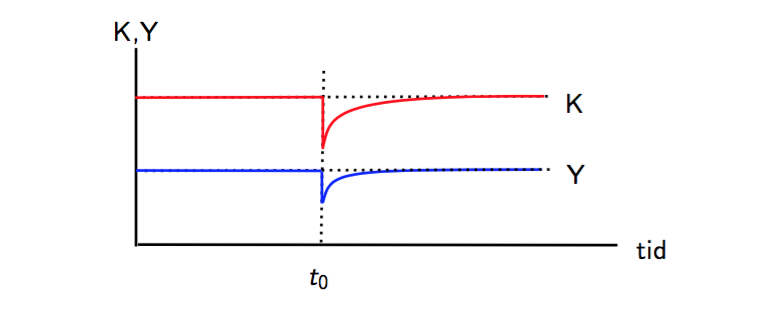
\includegraphics[scale=0.6]{skarm3}

\textbf{Befolkningsökning och teknisk utveckling} \par \noindent Den tillväxt som sker i befolkning och teknisk utveckling beskrivs med $ n = \frac{\Delta N}{N} \ g =  \frac{\Delta E}{E} $. BNP växer i takt med befolkning och teknsik utveckling. Detta på lång sikt. Med tillväxt så förväntar sig konsumenterna en högre inkomst imorgon, de spenderar mer idag, men alla kan inte låna mer i en sluten ekonomi. \par \noindent Konsumenterna måste "mutas" att inte spendera mer idag. \par

\textbf{Algoritm för att bestämma långsiktig BNP/capita: }
\begin{enumerate}
 \item Bestäm $ y = \frac{Y}{EN} $
 \item Sätt in med optimal kapitalstock, ta ut $ k^* $
 \item Sätt in den ekvationen som fås för $ k^* $ i orginal ekvationen för $ y = \frac{Y}{EN} $ som ger $ Y^* = (k^*)^{\alpha}EN $
\end{enumerate}


\vspace{5mm}
\title{Föreläsning 8}
\vspace{5mm} \par \noindent 

Vi kan se tydliga skillnader mellan Nord- och Sydkorea, de ena är öppet och fritt medan de andra stängt och planekonomi. Syd är 20ggr rikare idag än Nord. Detta är direkt beroende på vilken typ av ekonomi. 

\begin{itemize}
    \item Privat kapital: maskiner, byggnader
    \item Offentligt kapital: infrastruktur
\end{itemize}

\textbf{Inkomstskillnader: } Dessa kan försklaras av, fysiskt kapital ca $ 20 $, humankapital mellan $ 10  \ till \ 30  $  resterande måste bero på något annat, E ,[procent].
Då teknologin i fattiga länder många gånger är väldigt låg så är deras BNP också lägre. De kan helt enkelt inte mäta sig med omvärlden på grund utav deras dåliga tillgång till teknik. 

\vspace{5mm}
\title{Föreläsning 9}
\vspace{5mm} \par \noindent 

\textbf{Arbetslöshet:} \par \noindent Frågan är här; Varför söker inte unga jobb? Är de för få platser? Är det för fås som slutar? Kompetenser varierar mellan personer, så gör också viljan att ha ett jobb.  \par \noindent  OLF: de är dem som står utanför arbetskraften, sjuka, studerande, och/eller pensionärer.  \par \noindent Frågan är; Hur stor är chansen att få jobb om du söker?  \par \noindent 
Andelen som söker jobb delat med den andel jobb som öppnas upp. 
$$
f \approx \frac{s}{\lambda u+s}
$$
Där \textbf{s} är den andel som som slutar varje månad.  \par \noindent 

\begin{itemize}
    \item $ \lambda$: Färre sökande per plats om de sökande är mindre aktiva.
    \item s: 3-4 ggr vanligare att byta jobb i Tyskland och USA.
    \item u: Fler som söker $ \Rightarrow $ svårare att får jobb. 
\end{itemize}

Chansen att få jobb är större då fler lämnar och/eller när låg arbetslöshet gäller. Arbetslöshet är ett problem för både samhälle och individen. Ekonomiska kostnader och psyko-social konsekvenser. Det är framförallt den långsiktiga arbetslösheten som är svår, denna kan leda till utanförskap, tappad kompetens, och lägre inkomst. Sverige finns många starka unioner (fackföreningar) dessa medför en högre arbetslöshet. Dessa har inte lika stor påverkan i andra länder så som USA. 

\begin{itemize}
    \item $\lambda f $ är andelen arbetslösa som får jobb under månaden.
    \item v är andelen arbetslösa som lämnar arbetskraften. 
\end{itemize}

x är andelen som lämnar arbetslösheten varje månad. Denna blir mindre varje månad. Till slut så resutlerar den i en geometrisk serie som ger den andra ekvationen.  

$$
 x = \lambda f + v 
$$
$$
\frac{1}{\lambda f + v}
$$

\vspace{5mm}
\title{Föreläsning 10}
\vspace{5mm} \par \noindent 

\textbf{Teorier om arbetslöshet:}
\vspace{5mm} \par \noindent Effektivitets-löneteorin handlar om hur företag sätter löner för att minimera kostnaden för ett givet antal anställda. Om det är låg arbetslöshet så har företagen incitament att höja löner. Detta då det finns få som söker jobben. Vice versa gäller vid hög arbetslöshet, då omvänt. 

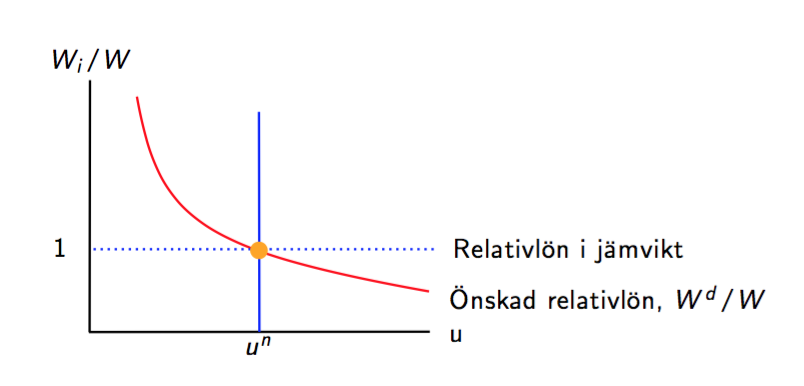
\includegraphics[scale=0.5]{skarm4}

Den önskade lönen blir där med: 
$$
W^d = (1+a+bu)W
$$
Vad skull ske på lång sikt om $ u < u^n$? \par \noindent 
Detta skulle medföra att $ N > N^n $. Det blir svårt att behålla och rekrytera personal. Se vad som händer på grafen. 

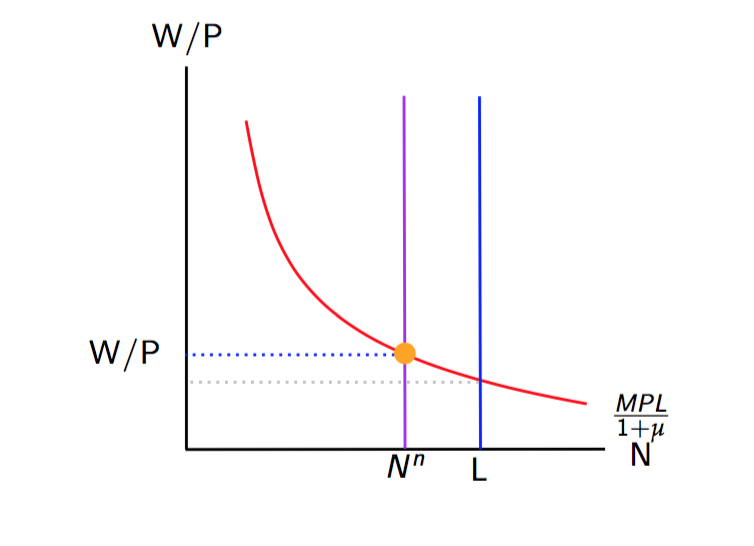
\includegraphics[scale = 0.5]{skarm5} \par

\textbf{Sökfriktioner} handlar om att arbetare har olika kvalitéer och preferenser. Det tar också tid att hitta rätt person till rätt jobb. De faktorer som påverkar graden av friktion och arbetslösheten är: \textbf{Intensiteten}, hur mycket och ofta de arbetslösa söker jobb. \textbf{Kräsenhet}, hur kräsna de är med vilket jobb de får, \textbf{Konkurrens}, hur väl de kan konkurera med andra på marknaden. Skulle inte sökfriktioner existera så skulle detta medföra att kurvan för $ u^n $ låg på en lägre nivå. Då sökfriktionerna medför att vissa inte får jobb, eller inte lika lätt i alla fall. Det vill säga sökfriktioner ökar på den naturliga arbetslösheten. Det finns visa vktiga faktorer för att påverka sökfriktioner. Dessa är sådan som: regler för arbetslöshetsersättning, utbildningssystmets förmåga att utrusta arbetskraft med färdigheter, och arbetsmarknadspolitikens utformning (arbetsförmedling osv). \par \noindent \vspace{5mm} \textbf{Appendix:} \par \noindent 
I Sverige existerar inte några minimelöner. Dock existerar det lägsta löner i de flesta kollektivavtal. Minimelöner kan medföra arbetslöshet speciellt för lågkvalificerade grupper. Den teknologiska utvecklingen kan vara en förklarande faktor till detta. Detta ger samma effekt som sökfriktioner. Större andel ställs utanför arbetsstyrkan. Länder med en generös arbetslöshetsersättning har högre arbetslöshet, detta kan bero på att de arbetslösa finner sig i att vara det. Därmed blir lata/bekväma. 

\vspace{5mm}
\title{Föreläsning 11}
\vspace{5mm} \par \noindent 

\textbf{Inflation och teori} \par \noindent \vspace{5mm}

Vad bestämmer efterfrågan på pengar? 
$$
M*V = P*Y 
$$
V: Velocity, hur ofta du får betalt, i princip. 
$$
M^d = \frac{1}{V} PY
$$
På lång sikt så kan vi se att prisnivån blir den övre formeln fast med substituerat $ i$. Inflationen om $r^n, \pi, V$ är konstant. Ger oss med hjälp av förenkling gjord i förelsäning 1 följande formel. 

$$ 
Y = Y^n: \ \pi = \frac{\Delta P }{P} = \frac{\Delta M}{M} - \frac{\Delta Y^n}{Y^n}
$$

Slutsatsen blir att om tillgången på pengar växer snabbare än jämviktsproduktionen så resulterar detta i inflation. Om landet försöker att finansiera offentliga utgifter till stor del med hjälp av att trycka mer pengar, det vill säga öka den monetära basen, så kommer det att resultera i en hyperinflation. Detta var vad som skede med Zimbabwe och Tyskland.  \par \noindent \vspace{5mm} 

\section{Korta sikten}
\vspace{5mm}
\title{Föreläsning 12}
\vspace{5mm} \par \noindent 

\textbf{IS-LM}
\vspace{5mm} \par \noindent 

IS-LM modellen har med Y som består av konsumtion och investeringar, samt realränta: $ r = i-\pi^e$. LM delen är funktionen för hur efterfrågan för pengar ser ut. IS ekvationen får vi från den avreagerade efterfrågan och den totala inkomsten. Den kan ses i nedanstående graf. Den långsiktiga inkomsten är helt vertikal, det vill säga beror inte alls i längden på efterfrågan. 

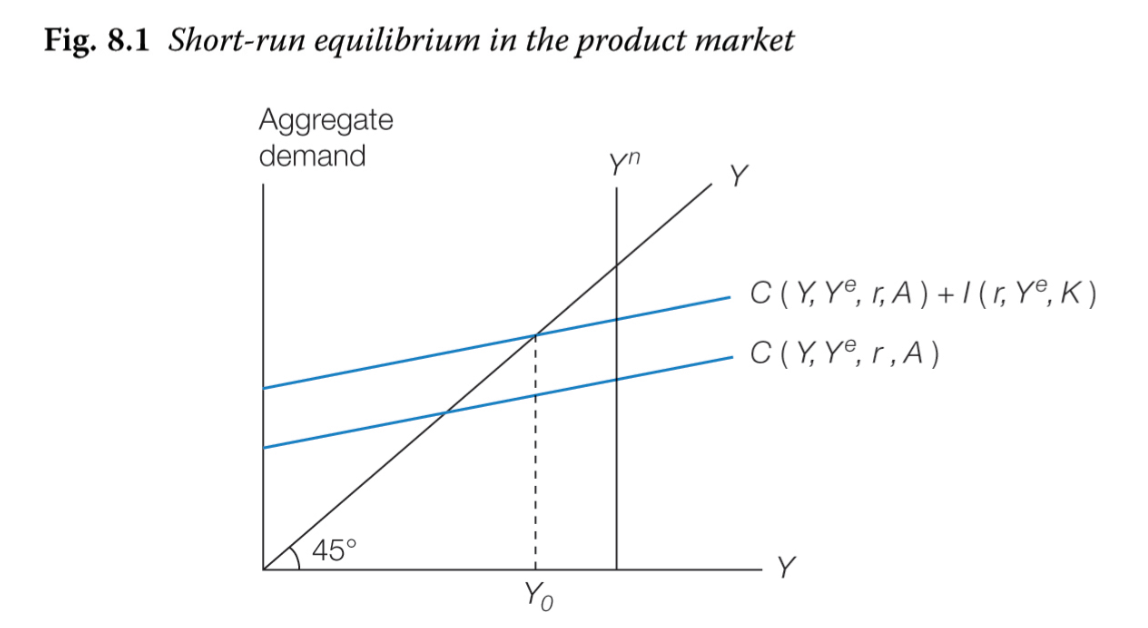
\includegraphics[scale=0.5]{skarm6} \vspace{5mm} \par \noindent 

\textbf{Multipliceringseffekten:} Den säger att vid en viss ändring $ \Delta I$ i aggregerad efterfrågan så sker en större ändring i $ Y$. En ökning i ränta medför en sänkning av konsumtion och investeringar. Detta kan ses i nedanstående bild. 

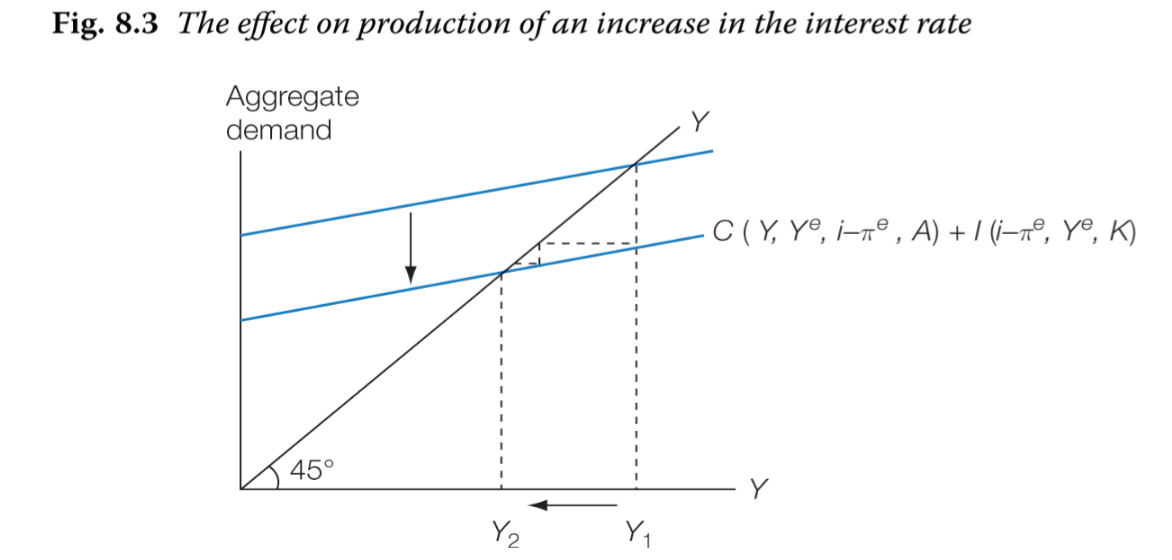
\includegraphics[scale=0.5]{skarm7} \vspace{5mm} \par \noindent 
Med hjälp av dessa får vi sedan den slutgiltiga IS-kurvan. Om den nominella räntan är lika med den naturliga realräntan och förväntad inflation så är också produktionen på den naturliga nivån. Ökar den nominella räntan så sjunker produktionen. \vspace{5mm} \par \noindent  Om det är så att utbudet på pengar ökar så minskar räntan. Detta går hand i hand med vår intuition. Det vill säga om det finns mer pengar på marknade, utbudet ökar, så sjunker efterfrågan på pengar och där med också hur mycket folk är villiga att betala för pengar. $\frac{M}{P}$ skiftar till höger. Om det istället är så att produktionen ökar så skiftar hela kurvan utåt. Detta för att ökar $\frac{Y}{V_i}$ så måste $\frac{M}{P}$ följa med (likhetstecken). IS-kurvan står för marknaden för varor och tjänster. LM-kurvan står för penningmarknaden. IS-LM modellen är en kortsiktig modell. Kom ihåg att alla modeller är fortfarande i slutna ekonomier. \vspace{5mm} \par \noindent Om personer blir mer optimistiska eller pessimistiska om framtiden så är det $ Y^e$ som ändrar sig och därför är det IS kurvan som skiftar utåt. Det är väldigt viktigt att identifiera och förklara vilken variabel som påverkas. 

\vspace{5mm}
\title{Föreläsning 14}
\vspace{5mm} \par \noindent 

\textbf{Inflation och arbetslöshet}
\vspace{5mm} \par \noindent 
Vad säger teorin om sambandet mellan arbetslöshet och inflation? Vi kan inte varaktigt ha en rabtslöshet som ligger under en viss jämviktsnivå utan att inflationen tar fart. Philipskurvan ger oss ett verktyg för att knyta ihop den långa och korta sikten. Vi har tre visioner av Philipskurvan. 
\begin{enumerate}
 \item Arbetslöshet och löneökning
 \item Arbetslöshet och prisinflation
 \item BNP-gap och prisinflation
\end{enumerate}

$$
   PC1:\ \frac{\Delta W_t}{W_{t-1}} = \frac{\Delta W^e_t}{W_{t-1}} - \hat{b}(u_t - u^n) 
$$
Där: $ \hat{b} = \frac{\lambda b}{1-\lambda}$
Den kurvan kan se ut på följande vis.

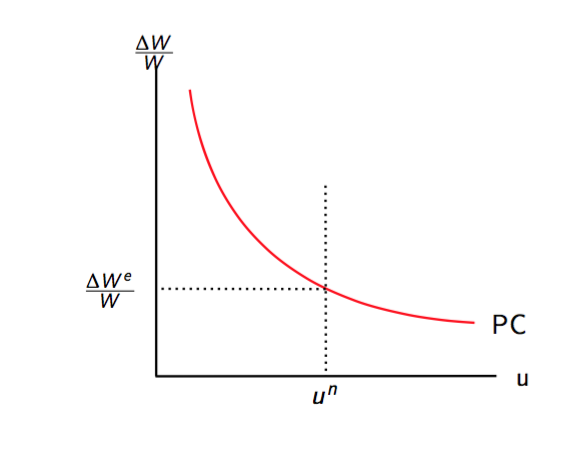
\includegraphics[scale=0.5]{skarm8}

$$
PC2: \ \pi = \pi^e - \hat{b}(u_t-u^n) + z
$$
Där Z = kostnadsstörningar. Den får representera alla typer av störningar på utbudsidan. Energipriser och skatter är exempel på sådana störningar. Högre kostnader ger högre $ \pi$.  \vspace{5mm} \par \noindent 

BNP gapet definieras i from av förändringen från det natruliga tillståndet. 
$$
\hat{Y} = \frac{Y-Y^n}{Y^n}
$$
Är detta positivt så ligger produktionen över jämviktsnivån och där med så ligger arbetslösheten under den naturliga nivån. Detta medför att löner ökar snabbare än väntat och att priser också stiger mer än väntat. Denna är den mest intressanta. Inflationen beror på BNP-gapet och kostnadschocker. Förväntningarna kommer från vad folket tror om framtiden. Det vill säga har det varit lågkonjuktur en längre tid så tror också folket att det kommer vara det nästa år. De blir försiktigare. 

$$
PC3: \ \pi = \pi^e + \beta \hat{Y} + z
$$
Kurvan kommer se ut som följande. 

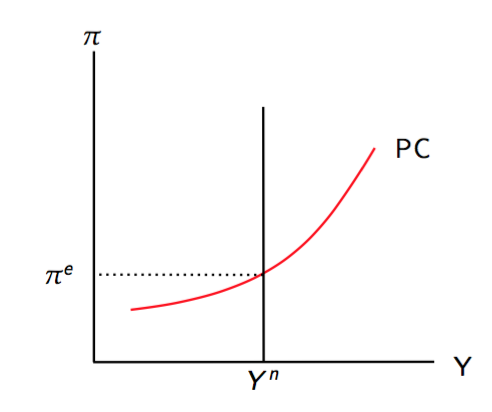
\includegraphics[scale=0.6]{skarm10} 
\vspace{5mm} \par \noindent 

Vi kan i princip har flera olika typer av förväntnigar av folket några av de vanliga är: 
\begin{enumerate}
 \item Backåtblickande: $ \pi^e_t = \pi_{t-1}$, dagens inflation är samma som igår 
 \item Trovärdigt inflationsmål: $ \pi^e_t = \pi^{\otimes}$
 \item Rationella förväntningar: $ \pi^e_t = \pi_t$ 
 \end{enumerate}

Vid en expansiv penningpolitik så rör vi oss endast längs med kurvan. Det flyttar inte på kurvan. Detta är period 1. Efter det så kommer folk att justera sina förväntningar och där med skifta kurvan uppåt. Om den landet fortsätter att föra en sådan politik så kommer händelsen att upprepa sig. Det vill säga inflationen fortsätter att stiga. Dock på väldigt lång sikt så går det inte att lura folk. Där med är den långsiktiga Philipskurvan helt vertikal. Det existerar ingen avvägning mellan aktivitet i ekonomin och inflation, det vill säga prisförändring. För att gå tillbaka till det ursprungliga läget så måste en restriktiv politik föras. \vspace{5mm} \par \noindent 

Vid ett trovärdigt inflationsmål så är den kortsiktiga och långsiktiga kurvan desamma. Vi rör oss med kurvan om det existerar en expansiv ekonomisk politik. \vspace{5mm} \par \noindent 

\textbf{Appendix:}\vspace{5mm} \par \noindent 
Idag verkar det som att många i Sverige har tilltro till inflationsmållet snarare än tillbakablickande syn. I Sverige så har arbetslösheten legat mellan $ 5-10 \%$ sedan 90-talet. Inflationen har också legat runt $ 2\%$. Som är målet.När inflationen väl är hög så tenderar den att fortsätta vara det då den förväntade inflationen är högre. 

\section{Ekonomisk politik}
\vspace{5mm}
\title{Föreläsning 15}
\vspace{5mm} \par \noindent 

\textbf{Penningpolitik på kort sikt}
\vspace{5mm} \par \noindent 
Vi knyter samman IS-LM och PC. För att se vad som händer på kortsikt vid olika scenarion. Penningpolitikens mål är att ha prisstabilitet i ekonomin. De har också andra mål som att hålla produktionen på en jämn nivå. Över lag stödja ekonomin. På kort sikt så existerar det en avvägning mellan låg inflation och arbetslöshet. Lång sikt finns ingen avvägning. 

\begin{itemize}
    \item Ökad optimism/pessimism = efterfrågestörning
    \item Råvaruprisfall = kostnadsstörning
    \item Fall i inflationsförväntningarna 
    \item Produktivitetsstörning
\end{itemize}

Så här startar vi i vår modell: 

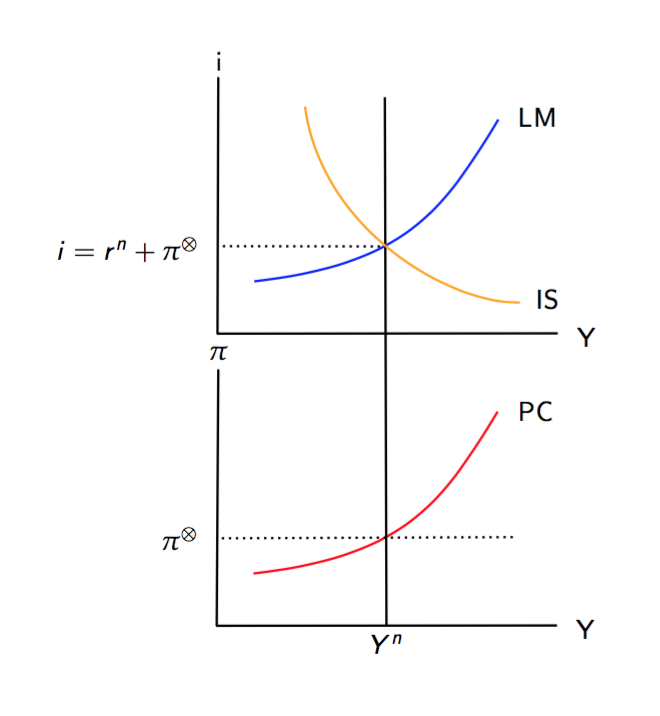
\includegraphics[scale=0.5]{skarm11} 

\vspace{5mm} \par \noindent 

Vi en negativ efterfrågestörning så flyttar IS inåt. Om inte banken agerar så kommer inflationen att sjunka längs PC. \vspace{5mm} \par \noindent Om det sker en kostnadsstörning så påverkar den PC i en period sedan så skiftar PC tillbaka till ursprungligt läge. Här kan banken reagera på två sätt, låta inflationen stiga för att $ Y^n = Y $ eller fösöka hålla nere inflationen via en stor ökning i räntan. Det vill säga $ i_1 = r' + \pi^{\otimes} $. 

\vspace{5mm} \par \noindent 

Vid en minskad inflationsförväntning så sjunker $ \pi^e < \pi^{\otimes} $. Detta påverkar först ränta som kommer att öka, detta skiftar IS inåt. För utom IS så skiftar också PC ner för att $ \pi^e$ är lägre än målet. Om inte banken agerar så kommer inflationen vara lägre och lika så BNP. Vid detta läget så måste räntan sänkas kraftigt för att nå tillbaka till $ \pi^{\otimes}$. 

\vspace{5mm} \par \noindent 

Det finns flera försvårade faktorer som riksbanken måste handskas med. 
\begin{itemize}
     \item Viss data blir först tillgänglig inom 0,5-1 år. 
     \item Penningpolitiken påverkar produktion och inflation med tidsfördröjning, 1-2 år. 
\end{itemize}

\textbf{Appendix: } \vspace{5mm} \par \noindent Är det så att arbetskraften blir mindre produktiv så är det ett skifte i E, detta av negativ from. Företagens kostnader ökar, det medför högre inflation. PC skiftar uppåt. Om banken i detta läge bryr sig mycket om inflationsmålet så kommer de att höja räntan. Detta medför att högkonjukturen fördjupas ytterligare. 
\vspace{5mm} \par \noindent 
\title{Föreläsning 16}
\vspace{5mm} \par \noindent 

\textbf{Finnanspolitik}

\vspace{5mm} \par \noindent 


Stora delar av Sveriges skatter kommer från direkta skatter på arbete och indirekta skatter på arbete. Mervärdesskatt är också en stor del av skatterna. De ofentliga utgifterna är uppdelade i många områden, några av de stora är Socialtskydd, Utbildning, Hälsa/Sjukvård och Infrastruktur. 

Den ofentliga sektorns budget resptrektion ser ut på följande vis: 
$$
\Delta D_{t-1} = G_t -T_t + rD_t 
$$

Förändringen i skuld = Statens konsumtion och investeringar - Skatter och transfereringar + Ränta på nuvarande skuld

$$
G-T = Primära \ budgetunderskottet 
$$
Ovanstående kan tolkas, hur mycket som spenderas - hur mycket inkomst som staten får. Detta betyder lever landet ovanför sina tillgångar eller spenderar de mindre än sina tillgångar. 

\vspace{5mm} \par \noindent 

Sverige har en relativt låg bruttoskuld jämfört med andra länder. Denna ligger på ungefär 40 \% av BNP:n. Tyskland som är ett starkt land har en skuld som ligger på hela 80 \%. Grekerna som har haft det svårt under en längre tid ligger på ca 170 \% av BNP. 

$$
d_t = \frac{D_t}{Y_t}
$$
Formeln ovan ger oss hur stor skulden är jämfört mot landets BNP. 
\vspace{5mm} \par \noindent Förändringen i med realränta: 
$$
\Delta d_{t+1} = \frac{G_t-T_t}{Y_t} + (r-g)\frac{D_t}{Y_t}
$$
Detta ger en formel som ser ut på följande vis. Denna formel är förändringen i skuld av BNP. 
$$
\Delta \frac{D}{Y} = \frac{G-T}{Y} + (r-g)\frac{D}{Y}
$$
Här ser vi då tydligt att, tillväxt reducerar skuldkvoten likaså gör en hög skatt eller ett lågt spenderade av staten. För att skuldration skall vara stabil måste villkoret nedan hålla.
$$
\Delta \frac{D}{Y} = 0
$$
Formeln för statens skuldtillväxt kan också skrivas i nominella termer. Se nedan.
$$
\Delta \frac{D}{Y} \approx \frac{G-T-iD}{Y} - (\pi + g)\frac{D}{Y} 
$$


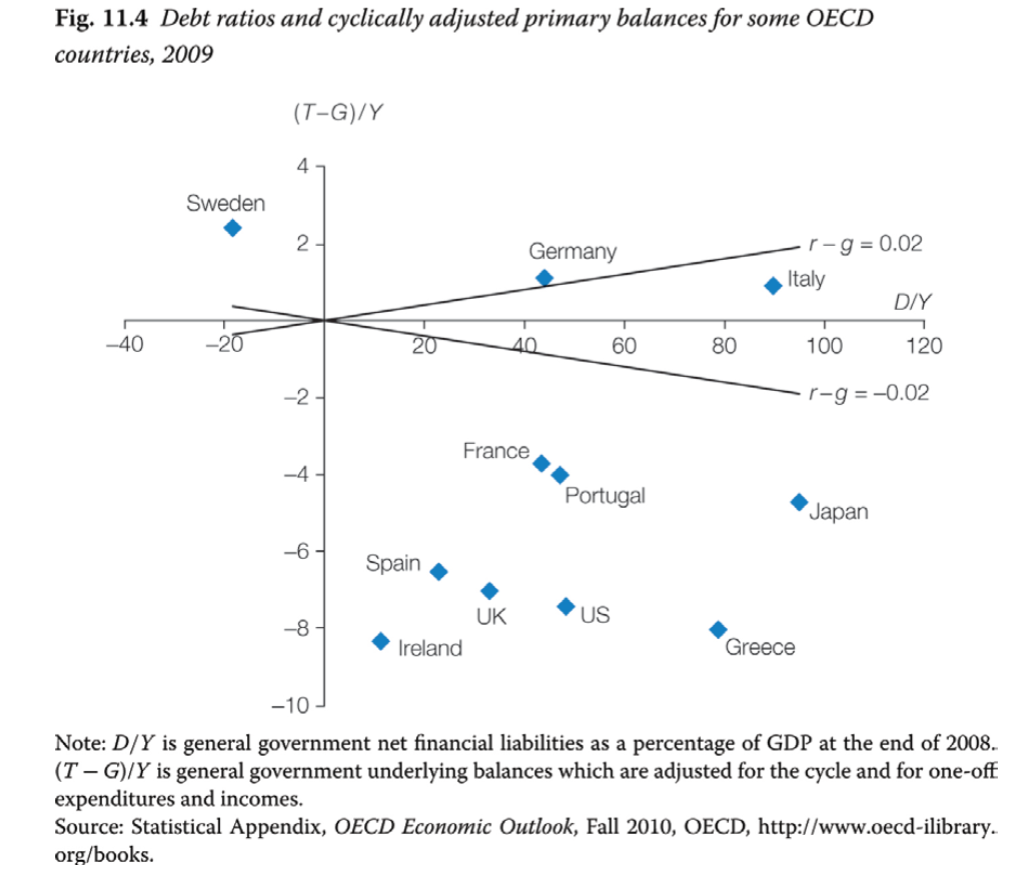
\includegraphics[scale=0.5]{skarm12}
\vspace{5mm} \par \noindent 
I bilden ovan ser vi vilka länder som har ett positivt primärt budgetunderskott och hur deras realränta är jämfört med tillväxtakten i landet. 

\vspace{5mm} \par \noindent 

Hushållens (reala) disponibla inkomst: $ Y^d = Y-T+rD $.  \par \noindent
Konsumptionsfunktionen inkluderat skatt: $  C_t = C(Y^t,Y^e-T^e,i-\pi^e, A) $. Där $ T^e $ är förväntad framtida skatt.

IS-LM inkluderat statlig konsumption: 
$$
Y = C(Y^t,Y^e-T^e,i-\pi^e, A) + I(i-\pi^e, Y^e,K) + G 
$$
LM ser likadan ut som tidigare. 
\vspace{5mm} \par \noindent 
En ökning av offentliga utgifter får ett större utslag på BNP än en reduktion av skatter. Reduceras skatterna så spenderar folket endast en andel av den ökade inkomsten. Den Rikardianska ekvivalensen säger att det spelar ingen roll hur en stat finansierar sina utgifter, antingen via ökade skatter eller lån. Befolkningen kommer annpassa sig till den förväntade framtiden. 

\vspace{5mm} \par \noindent 

Den nominella skuldration och reala skuldration kan sättas lika med varandra. 
\section{Den öppna ekonomin}
\vspace{5mm} \par \noindent 
\title{Föreläsning 18}
\vspace{5mm} \par \noindent 

\textbf{Nominell växelkurs: e}
\begin{itemize}
     \item Pris på inhemsk valuta i termer av utländsk valuta. 
     \item EUR/SEK
\end{itemize}
\vspace{5mm} \par \noindent 
\textbf{Real växelkurs: $ \varepsilon $}
\begin{itemize}
     \item Pris för inhemskt producerad vara i termer av utländsk producerad vara. 
\end{itemize}

Den reala växelkursens formel ses nedan: 
$$
\varepsilon = e * \frac{P}{P^*}
$$
Vi har nu tre olika ekvationer för aggregerad efterfrågan; AD. 
\begin{enumerate}
 \item Ekonomi utan stat, sluten. $ AD  = C + I $
 \item Ekonomi med stat, sluten. $ AD = C + I + G $
 \item Ekonomi med stat, öppen. $ AD = C + I + G + NX $ 
\end{enumerate}

Vad händer med nettoexporten om reala växelkursen stiger ? \vspace{5mm} \par \noindent  \textbf{1. }Den exporterade volymen sjunker som en faktor av att våra varor blir dyrare i utlandet. \textbf{2. }Vår krona stärks och vi kan köpa in mer av utlandet än innan. \textbf{3.}Det i sig medför att vår import ökar. \textbf{4. } Vi kan då anta att NX faller. $ \frac{dNX}{d \varepsilon} < 0 $. 

\vspace{5mm} \par \noindent 

IS i en öppen ekonomi påverkas av NX också. Det vill säga IS-kurvan kan skifta pågrund av fler faktorer. Tillexempel så ger en ändring av reala växelkursen ett skifte av IS. 

\textbf{Räteparitetsvillkoret}

\begin{itemize}
     \item NX beror på växelkursen.
     \item C och I beror på räntan. Konsumtion och investeringar sjunker med en ökad ränta. 
\end{itemize}

Räteparitet är sambandet mellan växelkurs och ränta. Ses nedan. 
$$
1+ i^*_t = (1+i_t) \frac{e_{t+1}^e}{e_t}
$$
Om landet i fråga använder sig av en fast och fullständigt trovärdig växelkurs medför detta följande: 
$$
e_{t+1}^e = e_t = e^\otimes
$$
$$
\Rightarrow i^*_t = i_t 
$$
Den nominella räntan i Sverige måste vara densamma som omvärlden. \vspace{5mm} \par \noindent Vid en flytande växelkurs så kommer dagens växelkurs anpassa sig till vad marknaden vill. Det ger oss följande formel. 
$$
1+ i^*_t = (1+i_t) \frac{e_{t+1}^e}{e_t}
$$
$$
\Rightarrow e_t = \frac{1+i_t}{1+i_t^*} e_{t+1}^e
$$
Approximation av ränteparitetsvillkoret: 
$$
i_t - i^*_t \approx - \frac{\Delta e^e_{t+1}}{e_t}
$$
Växelkursen här bestäms av framtida förväntad växelkurs, inhemsk nominell ränta och utländsk nominell ränta. Ränteskillnader kompenserar för den förväntade depricering/appriceringen av valutan. Om en förväntad depricering förutspås med 5 \% måste vår ränta vara 5 \% högre. \vspace{5mm} \par \noindent Om inverterare anser att sannolikheten för devalvering inte är 100 \% då så kommer räntan beror på hur troligt investerare anser att en devalvering kommer att ske. Det medför att räntan kommer att anpassas där efter. 

\vspace{5mm} \par \noindent

\textbf{Appendix}
\vspace{5mm} \par \noindent
Bytesbalansen = nationens finansiella sparande
\vspace{5mm} \par \noindent

Netto av bytesbalansen finansieras genom lån/till från andra länder genom köp/försäljning av tillgångar. 

$$
Bytesbalansen = fin.saprande = ökande/minskande \ nettofodringar = \Delta F 
$$
Med antagandet: $ Y^F + Tr^F = rF +0$ får vi följande formel. 
$$
\Rightarrow \Delta F = NX + rF 
$$
Sätter vi samman denna formel med DBNI så får vi formeln nedan. 
$$
\Delta F = Y + rF - C - G-I 
$$
Hur  bytesbalansen påverkas av inkomsten kan vi inte säga då $ Y $ bestäms endogent. 

\vspace{5mm} \par \noindent 
\title{Föreläsning 19}
\vspace{5mm} \par \noindent 

\textbf{Öppen ekonomi på långsikt}

\vspace{5mm} \par \noindent 
I den öppna ekonomin på lång sikt så är vi intresserade av att förstå vilka faktorer som bestämmer
\begin{itemize}
     \item Realränta
     \item Bytesbalansen
     \item Reala växelkursen
     \item Kapitalstocken och produktion
\end{itemize}

I en långsiktig jämvikt med konstant real växelkurs så ser formeln ut som nedan: 
$$
\frac{\Delta e}{e} = \pi^* - \pi
$$
Om ett litet öppet land har en högre inflation än omvärlden måste valutan falla för att konkurrenskraften ska bibehållas. Detta kan fås utifrån förändringen av nominella räntan. Använd förenkling från föreläsning 1.  Realräntan måste vara samma i det lilla landet som omvärlden. 

\vspace{5mm} \par \noindent 

\textbf{Kapitalstocken och produktion}
\vspace{5mm} \par \noindent 

Ett land bör investera så länge som nettomarginalavkastningen på kapital är högre än avkastningskravet på världsmarknaden. Om hushållens sparande inte räcker till så är det optimalt att låna in resten från utlandet. Det ger oss: 
$$
Y^n = F(K,EN^n) = f(k^*)EN^n
$$
Sparande och investeringar är inte nära relaterade med varandra. Länder kan ha stora investeringar genom lånat kapital från omvärlden. 

\begin{figure}
    \centering
    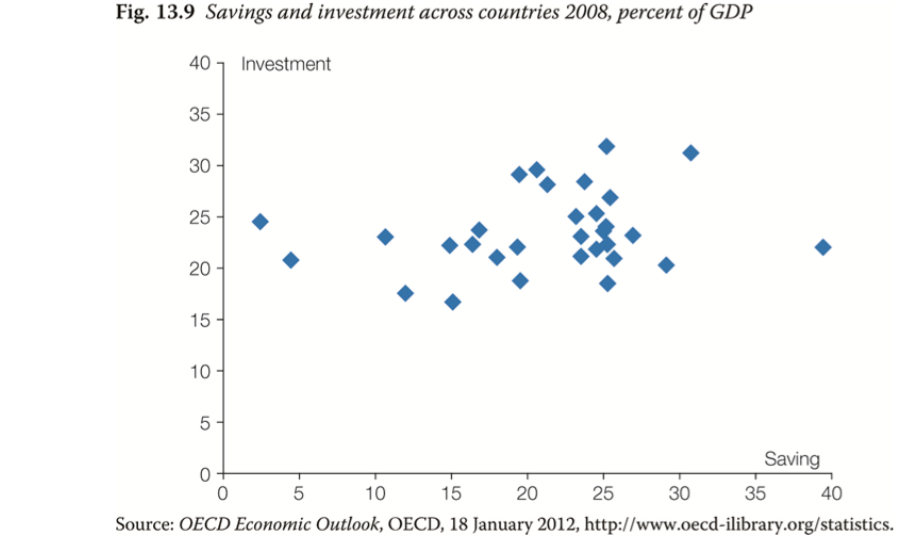
\includegraphics[scale=0.5]{skarm13}
    \caption{Figur över sparande och investeringar. Hade de varit nära relaterade hade vi set en 45 gradig linje}
    \label{fig:1 }
\end{figure}

I bilden nedan ser vi den reala växelkursen som ger en naturlig BNP. $ AD = Y^n$. 


 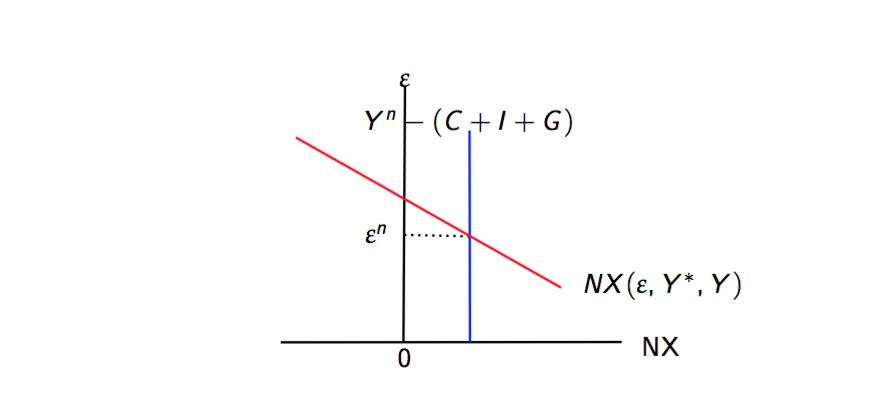
\includegraphics[scale=0.7]{skarm14}
 
Vid ökad pessimism om framtiden så leder det till en minskad investeringsvilja. Minskad investeringsvilja leder till en minskad inhemsk efterfrågan. Detta medför att konsumtion och investeringar minskar där med förskjuter C + I + G neråt. Detta medför en ökning av NX. 

\vspace{5mm} \par \noindent 

\textbf{Utlandsskuld på långsikt}
\vspace{5mm} \par \noindent 

Vad händer när konsumenter blir mer otåliga? De är trötta på att spara och vill istället leva loppan. De ökar därmed sin konsumtion. I detta fall då statsbdgeten är i balans och ingentillväxt existerar så kan konsumtionen endast öka om de använder mer än sin inkomst. Kapitaltillskottet måste då komma från omvärlden. Det vill säga bytesblansen blir negativ: $ \Delta < 0 $. 

Illustration nedan.



\bibliographystyle{plain}
\bibliography{references}

\end{document}
